\documentclass[margin={1pt 5mm 1pt 2mm},svgnames]{standalone}
\usepackage{fontspec}
\usepackage{tikz}
%\usepackage{amsmath}
%\usepackage{textgreek}
%\usepackage[version=4]{mhchem}
\usepackage{mathtools}

\setmainfont{TeX Gyre Heros}
\usetikzlibrary{arrows.meta, backgrounds, calc, fit, positioning, shapes}

\begin{document}
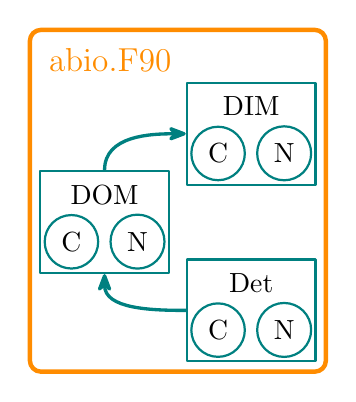
\begin{tikzpicture}[baseline=(abio.center), >={Stealth[round]}, line join=round, remember picture]
  \node (dim) [draw=Teal, thick, align=center, text width=14mm, text height=2ex, text depth=5ex] {DIM}; %, fill=Gray!20, 
  \node at (dim.south east) [above left=1.5ex, circle, draw=Teal, thick] {N};
  \node at (dim.south west) [above right=1.5ex, circle, draw=Teal, thick] {C};
  \node (dom) [below left=-2mm and 2mm of dim, draw=Teal, thick, align=center, text width=14mm, text height=2ex, text depth=5ex] {DOM}; %, fill=Gray!20
  \node at (dom.south east) [above left=1.5ex, circle, draw=Teal, thick] {N};
  \node at (dom.south west) [above right=1.5ex, circle, draw=Teal, thick] {C};
  \node (det) [below right=-2mm and 2mm of dom, draw=Teal, thick, align=center, text width=14mm, text height=2ex, text depth=5ex] {Det}; %, fill=Gray!20
  \node at (det.south east) [above left=1.5ex, circle, draw=Teal, thick] {N};
  \node at (det.south west) [above right=1.5ex, circle, draw=Teal, thick] {C};
  \node (abiof) at (dom.west|-dim.north) [above right, font=\large, DarkOrange] {abio.F90};
  \node (abio) [fit=(abiof) (dom) (det), draw=DarkOrange, ultra thick, rounded corners] {};
  \draw [->, very thick, Teal, out=90, in=180] (dom) to (dim);
  \draw [->, very thick, Teal, out=180, in=-90] (det) to (dom);
\end{tikzpicture}
\hspace*{5mm}
\begin{tikzpicture}[baseline=(phy.center), >={Stealth[round]}, line join=round, remember picture]
  \pgfdeclarelayer{background}
  \pgfsetlayers{background,main}
  % FS
  %\node (fsn) [circle, draw=Teal, thick] {N};
  %\node (fs) [above=1mm of fsn, inner sep=1pt] {Phy-FS};
  %\node (fsc) [below left=12mm and 5mm of fsn, circle, draw=Teal, dashed, thick] {C};
  %\node (fschl) [below right=12mm and 2mm of fsn, ellipse, draw=Teal, dashed, thick] {Chl};
  %\node (fsq) at ($(fsn)!0.5!(fsc)$) [draw, minimum width=3ex, text depth=0ex, text height=1.5ex] {Q};
  %\node (fst) at ($(fsn)!0.5!(fschl)$) [draw, minimum width=3ex, text depth=0ex, text height=1.5ex] {$\theta$};
  %\draw [->, thin, line cap=rect] (fsn) -- (fsq) -- (fsc);
  %\draw [->, thin, line cap=rect] (fsn) -- (fst) -- (fschl);
  % DA
  \node (dan) [circle, draw=Teal, thick] {N}; %[right=25mm of fsn]
  \node (da) [above=1mm of dan, inner sep=1pt] {Phy-DA};
  \node (dac) [below left=12mm and 5mm of dan, circle, draw=Teal, thick] {C};
  \node (dachl) [below right=12mm and 2mm of dan, ellipse, draw=Teal, dashed, thick] {Chl};
  \node (daq) at ($(dan)!0.5!(dac)$) [circle, draw=Teal, dashed, thick, inner sep=1pt, minimum width=3ex, text depth=0ex, text height=1.5ex] {Q};
  \node (dat) at ($(dan)!0.5!(dachl)$) [circle, draw=Teal, dashed, thick, inner sep=1pt, minimum width=3ex, text depth=0ex, text height=1.5ex] {$\theta$};
  \draw [->, thick, line cap=rect] (dan) -- (daq);
  \draw [->, thick, line cap=rect] (dac) -- (daq);
  \draw [->, thick, line cap=rect] (dan) -- (dat) -- (dachl);
  \draw [->, thick, line cap=rect] (daq) -- (dat);
  % IA
  \node (ian) [right=25mm of dan] [circle, draw=Teal, dashed, thick] {N};
  \node (ia) [above=1mm of ian, inner sep=1pt] {Phy-IA};
  \node (iac) [below left=12mm and 5mm of ian, circle, draw=Teal, thick] {C};
  \node (iachl) [below right=12mm and 2mm of ian, ellipse, draw=Teal, dashed, thick] {Chl};
  \node (iaq) at ($(ian)!0.5!(iac)$) [circle, draw=Teal, dashed, thick, inner sep=1pt, minimum width=3ex, text depth=0ex, text height=1.5ex] {Q};
  \node (iat) at ($(ian)!0.5!(iachl)$) [circle, draw=Teal, dashed, thick, inner sep=1pt, minimum width=3ex, text depth=0ex, text height=1.5ex] {$\theta$};
  \draw [->, thick, line cap=rect] (iac) -- (iaq);
  \draw [->, thick, line cap=rect] (iaq) -- (ian);
  \draw [->, thick, line cap=rect] (ian) -- (iat) -- (iachl);
  \draw [->, thick, line cap=rect] (iaq) -- (iat);
  %\node (fsb) [fit=(fs) (fsc) (fschl), draw=Teal, thick] {}; %fill=Gray!20, 
  \node (dab) [fit=(da) (dac) (dachl), draw=Teal, thick] {}; %fill=Gray!20, 
  \node (iab) [fit=(ia) (iac) (iachl), draw=Teal, thick] {}; %fill=Gray!20, 
  \node (phyf) at (dab.north west) [above right, font=\large, DarkOrange] {phy.F90};
  \begin{pgfonlayer}{background}
    \node (phy) [fit=(phyf) (iab), draw=DarkOrange, ultra thick, rounded corners] {};
  \end{pgfonlayer}
  \draw [->, very thick, Teal, out=80, in=100, overlay, looseness=0.4] (dim) to (phy);
  \draw [->, very thick, Teal, out=-100, in=-80, overlay, looseness=0.4] (phy) to (det);
\end{tikzpicture}
\end{document}
